\section{Keccak-p Permutations}
\textsc{Keccak}-p is a fixed length permutation which is the underlying permutation (denoted earlier by $f$) used by the \textsc{sha-3} family of functions as specified by the NIST~\cite{NIST}. The steps of this permutation are described below, before defining the hash functions in their entirety in Section~\ref{section:sha3}.

\begin{defn} Two parameters are specified for a \textsc{Keccak}-p function:
  \begin{itemize}[label=\textperiodcentered,nolistsep]
  \item The \emph{width} of a permutation is the fixed length of the bit strings that are permuted.
    \item A \emph{round} is an iteration of an internal transformation.
  \end{itemize}
\end{defn}

For any $b$ in $ \{25, 50, 100, 200, 400, 800, 1600\} $ and any positive integer $n_r$, \textsc{Keccak}-p $\lbrack b, n_r \rbrack$ denotes the \textsc{Keccak}-p permutation of \emph{width} $b$ with $n$ \emph{rounds}.

A round of a \textsc{Keccak}-p permutation, denoted by \textsc{Rnd}, consists of a sequence of five transformations, called the \emph{step mappings}. The permutation is specified in terms of the values of the state. The state is initially set to the
input values of the permutation.
\subsection{The State}
For the sake of simplicity and to help understanding we shall limit our study to the case where $b=50$.
The NIST standard specifies two other quantities related to $b$: $w=b/25$ and $l = \log_2{b/25}$. In our case $l = 1$ and $w=2$.

The state of the \textsc{Keccak}-p permutation can be represented either:
\begin{itemize}
\item as a string whose bits are indexed from 0 to $b-1$. $S=S\lbrack 0 \rbrack \vert \vert S\lbrack 1 \rbrack \vert \vert S\lbrack 2 \rbrack \vert \vert \cdots S\lbrack b-1 \rbrack$
\item as a \emph{state array} which is a three dimensional array representation of the state \textbf{A}. A is a 5-by-5-by-$w$ array of bits. And $A\lbrack x,y,z \rbrack$ corresponds to the bit $(x,y,z) \in \llbracket 0,5 \llbracket \times \llbracket 0,5 \llbracket \times \llbracket 0,w \llbracket$.
\end{itemize}
In figure~\ref{fig:StateArray}, the different parts of a \textsc{Keccak}-p permutation state array are represented.

The two-dimensional parts of the array are called \emph{sheets}, \emph{planes} and \emph{slices}.

The single-dimensional parts of the array are called \emph{rows}, \emph{columns}, and \emph{lanes}.

\begin{figure}[H]
\centering
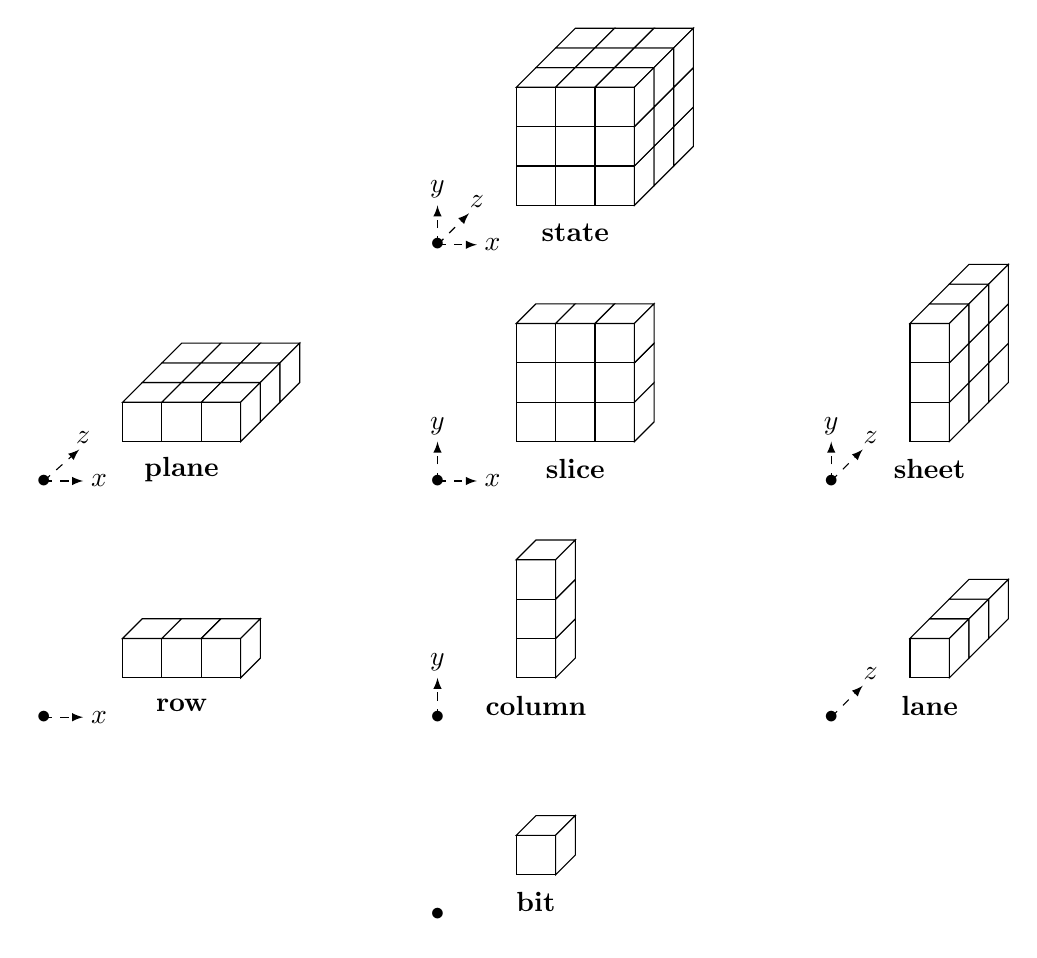
\begin{tikzpicture}[scale=0.5]

\newcommand\xaxis{1}
\newcommand\yaxis{1}
\newcommand\zaxis{1}
  
\newcommand\faceside[6]{
  \draw (-2+#4,-1+#5) node[]{} node{$\bullet$};
  \pgfmathparse{#1/2+#4}
  \node[text centered, font=\bf] at (\pgfmathresult,-0.7+#5) {#6};
  \foreach \a in {1,...,#1} {
    \foreach \b in {1,...,#2} {
      \fill[fill=white, draw=black] (#4+-1+\a,#5+-1+\b) -- (#4+\a,#5+-1+\b) -- (#4+\a,#5+\b) -- (#4+-1+\a,#5+\b) -- cycle;
    }
    \pgfmathparse{-1+#3}
    \foreach \d [evaluate=\d as \dd using \d*0.5] in {0,...,\pgfmathresult} {
      \fill[fill=white, draw=black] (#4+-1+\a+\d-\dd,#5+#2+\d-\dd) -- (#4+\a+\d-\dd,#5+#2+\d-\dd) -- (#4+\a+\d+0.5-\dd,#5+#2+\d+0.5-\dd) -- (#4+\a+\d-0.5-\dd,#5+#2+\d+0.5-\dd) -- cycle;
    }
  }
  \foreach \c in {1,...,#2} {
    \pgfmathparse{-1+#3}
    \foreach \e [evaluate=\e as \ee using \e*0.5] in {0,...,\pgfmathresult} {
      \fill[fill=white, draw=black] (#4+#1+\e-\ee,#5+-1+\c+\e-\ee) -- (#4+#1+\e+0.5-\ee,#5+-1+\c+\e+0.5-\ee) -- (#4+#1+\e+0.5-\ee,#5+0.5+\c+\e-\ee) -- (#4+#1+\e-\ee,#5+\c+\e-\ee) -- cycle;
      }
  }
}

\faceside{1}{1}{1}{10}{0}{bit}
\faceside{3}{1}{1}{0}{5}{row}\draw [->, >=latex, dashed] (-2,4) -- (-1,4);\draw (-0.6,4) node[]{$x$};
\faceside{1}{3}{1}{10}{5}{column}\draw [->, >=latex, dashed] (8,4) -- (8,5);\draw (8,5.4) node[]{$y$};
\faceside{1}{1}{3}{20}{5}{lane}\draw [->, >=latex, dashed] (18,4) -- (18.8,4.8);\draw (19,5.1) node[]{$z$};
\faceside{3}{1}{3}{0}{11}{plane}\draw [->, >=latex, dashed] (-2,10) -- (-1,10);\draw [->, >=latex, dashed] (-2,10) -- (-1.1,10.8);\draw (-0.6,10) node[]{$x$};\draw (-1,11.1) node[]{$z$};
\faceside{3}{3}{1}{10}{11}{slice}\draw [->, >=latex, dashed] (8,10) -- (9,10);\draw [->, >=latex, dashed] (8,10) -- (8,11);\draw (9.4,10) node[]{$x$};\draw (8,11.4) node[]{$y$};
\faceside{1}{3}{3}{20}{11}{sheet}\draw [->, >=latex, dashed] (18,10) -- (18,11);\draw [->, >=latex, dashed] (18,10) -- (18.8,10.8);\draw (18,11.4) node[]{$y$};\draw (19,11.1) node[]{$z$};
\faceside{3}{3}{3}{10}{17}{state}\draw [->, >=latex, dashed] (8,16) -- (9,16);\draw [->, >=latex, dashed] (8,16) -- (8,17);\draw [->, >=latex, dashed] (8,16) -- (8.8,16.8);\draw (9.4,16) node[]{$x$};\draw (8,17.4) node[]{$y$};\draw (9,17.1) node[]{$z$};

\end{tikzpicture}
\caption{\label{fig:StateArray}The parts of the state array for $x,y,z \in\llbracket 0,3 \llbracket \times \llbracket 0,3 \llbracket \times \llbracket 0,3 \llbracket$ }
\end{figure}

We shall label our state arrays in such a way that the lane that corresponds to (x,y) = (0,0) is in the center of the slices, as in~\ref{fig:LabelStateArray}

\begin{figure}[H]
\centering
\includegraphics[width=0.5\textwidth]{img/LabelStateArray.png}
\caption{\label{fig:LabelStateArray}Convention for the coordinates of the state array.}
\end{figure}

The correspondance between the string reprsentation of the state and the state array is defined as follows:

For $(x,y,z) \in \llbracket 0,5 \llbracket \times \llbracket 0,5 \llbracket \times \llbracket 0,w \llbracket$,
$$A\lbrack x,y,z \rbrack=S\lbrack w\cdot (5y+x)+z \rbrack.$$



In our example $b=50$, therefore $w=2$, which gives us:
$$A\lbrack x,y,z \rbrack=S\lbrack 2\cdot (5y+x)+z \rbrack.$$

\begin{equation}
\begin{aligned}
A \lbrack 0,0,0\rbrack = S\lbrack 0 \rbrack & \hspace{2cm} A \lbrack 1,0,0\rbrack = S\lbrack 2 \rbrack & \hspace{2cm} \ldots & \hspace{2cm} A \lbrack 4,0,0\rbrack = S\lbrack 8 \rbrack\\
A \lbrack 0,0,1\rbrack = S\lbrack 1 \rbrack & \hspace{2cm} A \lbrack 1,0,1\rbrack = S\lbrack 3 \rbrack & \hspace{2cm} \ldots & \hspace{2cm} A \lbrack 4,0,1\rbrack = S\lbrack 9 \rbrack\\
\end{aligned}
\end{equation}

and

\begin{equation}
\begin{aligned}
A \lbrack 0,1,0\rbrack = S\lbrack 10 \rbrack & \hspace{2cm} A \lbrack 1,1,0\rbrack = S\lbrack 12 \rbrack & \hspace{2cm} \ldots & \hspace{2cm} A \lbrack 4,1,0\rbrack = S\lbrack 18 \rbrack\\
A \lbrack 0,1,1\rbrack = S\lbrack 11 \rbrack & \hspace{2cm} A \lbrack 1,1,1\rbrack = S\lbrack 13 \rbrack & \hspace{2cm} \ldots & \hspace{2cm} A \lbrack 4,1,1\rbrack = S\lbrack 19 \rbrack\\
\vdots                                       & \hspace{2cm} \vdots                                       & \hspace{2cm} \vdots & \hspace{2cm} \vdots                                    \\
A \lbrack 0,4,0\rbrack = S\lbrack 40 \rbrack & \hspace{2cm} A \lbrack 1,4,0\rbrack = S\lbrack 42 \rbrack & \hspace{2cm} \ldots & \hspace{2cm} A \lbrack 4,4,0\rbrack = S\lbrack 48 \rbrack\\
A \lbrack 0,4,1\rbrack = S\lbrack 41 \rbrack & \hspace{2cm} A \lbrack 1,4,1\rbrack = S\lbrack 43 \rbrack & \hspace{2cm} \ldots & \hspace{2cm} A \lbrack 4,4,1\rbrack = S\lbrack 49 \rbrack\\
\end{aligned}
\end{equation}


The reverse operation, i.e.\ converting a state array representation to the string representation can be done using the lanes and planes of A.

Bits in a given lane follow sequencial order ($x=x, y=y, z=z+1$), and at the end of a lane, the following indexation of S if obtained by moving to the next lane in the same plane ($x=x+1, y=y, z=0$).
Once all the lanes in a plane have been explored, the following indexation of S is obtained by moving to the first lane of the next plane ($x=0, y=y+1, z=0$).

\begin{defn}
For $(x,y) \in \llbracket 0,5 \llbracket \times \llbracket 0,5 \llbracket$, the string \textbf{Lane (x,y)} is defined as:
$$Lane (x, y) = A\lbrack x, y, 0\rbrack \vert \vert A\lbrack x, y, 1\rbrack \vert \vert A\lbrack x, y, 2\rbrack \vert \vert \cdots \vert \vert A\lbrack x, y, w-2\rbrack \vert \vert A\lbrack x, y, w-1\rbrack $$
\end{defn}
In our example:
\begin{equation}
\begin{aligned}
Lane (0, 0) =& A\lbrack 0, 0, 0\rbrack \vert \vert A\lbrack 0, 0, 1\rbrack \\
Lane (1, 0) =& A\lbrack 1, 0, 0\rbrack \vert \vert A\lbrack 1, 0, 1\rbrack \\
Lane (2, 0) =& A\lbrack 2, 0, 0\rbrack \vert \vert A\lbrack 2, 0, 1\rbrack \\
\vdots & \\
\end{aligned}
\end{equation}

\begin{defn}
For $ y \in \llbracket 0,5 \llbracket$, the string \textbf{Plane(y)} is defined as:
$$Plane (y) = Lane (0,y) \vert \vert Lane (1,y) \vert \vert Lane (2,y) \vert \vert Lane (3,y) \vert \vert Lane (4,y) $$
\end{defn}
And then
$$S= Plane (0) \vert \vert  Plane (1) \vert \vert Plane (2) \vert \vert  Plane (3) \vert \vert  Plane (4) $$

In our example:
\begin{equation}
\begin{aligned}
S = & A\lbrack 0, 0, 0\rbrack \vert \vert A\lbrack 0, 0, 1\rbrack \\
    & A\lbrack 1, 0, 0\rbrack \vert \vert A\lbrack 1, 0, 1\rbrack \\
    & A\lbrack 2, 0, 0\rbrack \vert \vert A\lbrack 2, 0, 1\rbrack \\
    & A\lbrack 3, 0, 0\rbrack \vert \vert A\lbrack 3, 0, 1\rbrack \\
    & A\lbrack 4, 0, 0\rbrack \vert \vert A\lbrack 4, 0, 1\rbrack \\
    & \\
    & A\lbrack 0, 1, 0\rbrack \vert \vert A\lbrack 0, 1, 1\rbrack \\
    & A\lbrack 1, 1, 0\rbrack \vert \vert A\lbrack 1, 1, 1\rbrack \\
    & A\lbrack 2, 1, 0\rbrack \vert \vert A\lbrack 2, 1, 1\rbrack \\
    & A\lbrack 3, 1, 0\rbrack \vert \vert A\lbrack 3, 1, 1\rbrack \\
    & A\lbrack 4, 1, 0\rbrack \vert \vert A\lbrack 4, 1, 1\rbrack \\
    & \vdots \\
    & A\lbrack 0, 4, 0\rbrack \vert \vert A\lbrack 0, 4, 1\rbrack \\
    & A\lbrack 1, 4, 0\rbrack \vert \vert A\lbrack 1, 4, 1\rbrack \\
    & A\lbrack 2, 4, 0\rbrack \vert \vert A\lbrack 2, 4, 1\rbrack \\
    & A\lbrack 3, 4, 0\rbrack \vert \vert A\lbrack 3, 4, 1\rbrack \\
    & A\lbrack 4, 4, 0\rbrack \vert \vert A\lbrack 4, 4, 1\rbrack \\
\end{aligned}
\end{equation}

\subsection{Step Mappings}
A round of \textsc{Keccak}-p$\lbrack b, n_r \rbrack$ is composed of five step mappings whose algorithms we shall develop below. They all take as input a state array A and output an updated state array. The last step mapping has an additional parameter which is the round index $i_r$.

\subsubsection{The First Step Function $\Theta$}
\begin{algorithm}[H]
\caption{$\Theta$ (A)}
\label{algo:Theta}
\begin{algorithmic}[1]
\For{$(x,z) \in \llbracket 0,5 \llbracket \times \llbracket 0,w \llbracket$}
\State{$C\lbrack x,z\rbrack = A\lbrack x, 0, z\rbrack \oplus A\lbrack x, 1, z\rbrack \oplus A\lbrack x, 2, z\rbrack \oplus A\lbrack x, 3, z\rbrack \oplus A\lbrack x, 4, z\rbrack $}
\EndFor{}

\For{$(x,z) \in \llbracket 0,5 \llbracket \times \llbracket 0,w \llbracket$}
\State{$D\lbrack x,z\rbrack = C\lbrack (x-1) \mod{5}, z\rbrack \oplus C\lbrack (x+ 1) \mod{5}, (z-1) \mod{w}\rbrack $}
\EndFor{}

\For{$(x,y,z) \in \llbracket 0,5 \llbracket \times \llbracket 0,5 \llbracket \times \llbracket 0,w \llbracket$}
\State{$A'\lbrack x, y, z\rbrack = A\lbrack x, y, z\rbrack \oplus D\lbrack x,z\rbrack$}
\EndFor{}

\Return{$A'$}
\end{algorithmic}
\end{algorithm}

Algorithm~\ref{algo:Theta}, which performs the first step mapping, starts by calculating the parity of each column of the state array, to be stored in variables $C\lbrack x,z\rbrack$ for all values of $x$ and $z$.

Then a new set of $5 \times w$ values is computed, each $D\lbrack x,z\rbrack$ representing the sum of the parity of two columns.

Finally each bit in the state is XOR-ed with a value of $D$ as illustrated in Figure~\ref{fig:Theta}.

\begin{figure}[H]
\centering
\includegraphics[width=0.3\textwidth]{img/Theta.png}
\caption{\label{fig:Theta}The effect of $\Theta$ on a bit of the state array.}
\end{figure}

\subsubsection{The Second Step Function $\rho$}
$\rho$ rotates each lane by an \emph{offset}, thus each lane is modified by adding the offset to the z coordinate, modulo the lane size $w$. The offset depends on the x and y coordinates of the given lane.
\begin{algorithm}[H]
\caption{$\rho$ (A)}
\label{algo:rho}
\begin{algorithmic}[1]
\For{$z \in \llbracket 0,w \llbracket$}
\State{$A'\lbrack 0, 0, z\rbrack = A\lbrack 0, 0, z\rbrack $}
\EndFor{}
\State{$(x,y) \gets (1,0)$}
\For{$t=0$ to $23$}
\For{$z=0$ to $w-1$}
\State{$A'\lbrack x, y,z\rbrack = A\lbrack x, y, (z-(t+1)\cdot (t+2)/2) \mod{w} \rbrack $}
\EndFor{}
\State{$(x,y) \gets (y, (2\cdot x + 3\cdot y) \mod{5})$}
\EndFor{}
\Return{$A'$}
\end{algorithmic}
\end{algorithm}

\subsubsection{The Third Step Function $\pi$}
$\pi$ rearranges the position of the lanes.
\begin{algorithm}[H]
\caption{$\pi$ (A)}
\label{algo:pi}
\begin{algorithmic}[1]
\For{$(x,y,z) \in \llbracket 0,5 \llbracket \times \llbracket 0,5 \llbracket \times \llbracket 0,w \llbracket$}
\State{$A'\lbrack x, y, z\rbrack = A\lbrack( x+ 3 \cdot y)\mod{5}, x, z\rbrack $}
\EndFor{}
\Return{$A'$}
\end{algorithmic}
\end{algorithm}

\subsubsection{The Third Step Function $\chi$}
$\chi$ XOR's each bit with a non linear function of two other bits in it's row.
\begin{algorithm}[H]
\caption{$\chi$ (A)}
\label{algo:chi}
\begin{algorithmic}[1]
\For{$(x,y,z) \in \llbracket 0,5 \llbracket \times \llbracket 0,5 \llbracket \times \llbracket 0,w \llbracket$}
\Comment{$\cdot$ is equivalent to a boolean AND operation.}
\State{$A'\lbrack x, y, z\rbrack = A\lbrack x, y, z\rbrack \oplus ((A\lbrack( x+ 1)\mod{5}, y, z\rbrack \oplus 1) \cdot A\lbrack (x+2)\mod{5}, y, z\rbrack )$}
\EndFor{}
\Return{$A'$}
\end{algorithmic}
\end{algorithm}

\subsubsection{The Final Step Mapping $\iota$}
The $\iota$ step mapping takes an additional parameter $i_r$ called the \emph{round index}. An auxiliary function $rc$, based on a linear feedback shift register, takes the round index as an input and calculates a \emph{round constant} $RC$. This round constant is then XORed to the \emph{Lane (0,0)} of the state.

\emph{Lane(0,0)} is the only lane that is affected by $\iota$.

\begin{algorithm}[H]
\caption{$rc$ (t)}
\label{algo:rc}
\begin{algorithmic}[1]
\If{$t \mod{255}=0$}
\Return{1}
\EndIf{}
\State{$R \gets 10000000$}
\For{$i=1$ to $t\mod{255}$}
\State{$R \gets 0 \vert \vert R$}
\State{$R\lbrack 0\rbrack \gets R\lbrack 0 \rbrack \oplus \lbrack 8 \rbrack$}
\State{$R\lbrack 4\rbrack \gets R\lbrack 4 \rbrack \oplus \lbrack 8 \rbrack$}
\State{$R\lbrack 5\rbrack \gets R\lbrack 5 \rbrack \oplus \lbrack 8 \rbrack$}
\State{$R\lbrack 6\rbrack \gets R\lbrack 6 \rbrack \oplus \lbrack 8 \rbrack$}
\State{$R=\lfloor R\rfloor _8$}
\EndFor{}
\Return{$R\lbrack 0\rbrack$}
\end{algorithmic}
\end{algorithm}

\begin{algorithm}[H]
\caption{$\iota$ (A, $i_r$)}
\label{algo:iota}
\begin{algorithmic}[1]
\For{$(x,y,z) \in \llbracket 0,5 \llbracket \times \llbracket 0,5 \llbracket \times \llbracket 0,w \llbracket$}
\State{$A'\lbrack x, y, z\rbrack = A\lbrack x, y, z\rbrack$}
\EndFor{}
\For{$j=0$ to $l$}
\State{$RC\lbrack 2^j-1\rbrack = rc(j+7\cdot i_r)$}
\EndFor{}
\For{$z \in \llbracket 0,w \llbracket$}
\State{$A'\lbrack 0, 0, z\rbrack = A'\lbrack 0, 0, z\rbrack \oplus RC\lbrack z \rbrack$}
\EndFor{}
\Return{$A'$}
\end{algorithmic}
\end{algorithm}

\subsection{The Keccak-p Function}
Given a state array A and a round index $i_r$, the round function \textsc{Rnd} is the transformation that results from applying the step mappings $\Theta$, $\rho$, $\pi$, $\chi$, and $\iota$, in that order.
$$\textsc{Rnd}(A,i_r)=\iota ( \chi ( \pi ( \rho (\Theta (A)))), i_r)$$

The $\textsc{Keccak}$-p$\lbrack b, n_r \rbrack$ permutation applies $n_r$ iterations of \textsc{Rnd}.
Algorithm~\ref{algo:keccak} describes the whole permutation, where the input is a bit-string $S$ of length $b$. The width $b$ and number of rounds $n_r$ are fixed parameters.
\begin{algorithm}[H]
\caption{$\textsc{Keccak}$-p$\lbrack b, n_r \rbrack$ (S)}
\label{algo:keccak}
\begin{algorithmic}[1]
  \State{$A \gets S$ converted into a state array}
  \For{$i_r \in \llbracket 12+2\cdot l -n_r, 12 + 2\cdot l -1 \llbracket$}
  \State{$A \gets \textsc{Rnd}(A,i_r)$}
  \EndFor{}
  \State{$S' \gets A$ converted into a bit string of length $b$}
\Return{$S'$}
\end{algorithmic}
\end{algorithm}
